\section{Subsystem decomposition}
The subsystem CalendarManagement is the system where most of the program is placed. This system is responsible for all the local events happening in the system. This means that it would handle creation of the calendar, events and provide the necessary GUI for the local program. 

This subsystem has two connections outside the subsystem itself. The first one goes to "ShareSubsystem" that has all the necessary functions that the CalendarManagement system could ask for when it is about to share a calendar or an event. The other outgoing connection is to the SyncSubsystem. This is an interface that holds all the needed method calls to synchronize the calendar.
\newline
\newline
The ShareSubsystem has to do with sending the information to the right people and using the right systems. The reason why we made this an interface is that it has been a commonly thing to share through facebook and other social media platforms. Therefore it would be nice to easily have the opportunity to extend the share option so that it would support e.g. Facebook. 
\newline
\newline
The subsystem SyncSubsystem is where we keep our calendars up to date, where we got the information, of whom the calendar belongs to, and which users that are invited to see it. The SyncSubsystem keep the client calendars synchronized and handles the updates between the local calendar and the online ones. This is also behind an interface so that we can easily exchange it. That would turn to our advantage so the maintenance and upgrades of the system could be done easy. You simply exchange the subsystem part with a new one. E.g. if we wanted to update our synchronization part with a newer version of a data base program, the SyncSubsystem is exchanged, but the rest could stay intact. 
\newline
\begin{figure}[h]
\centering
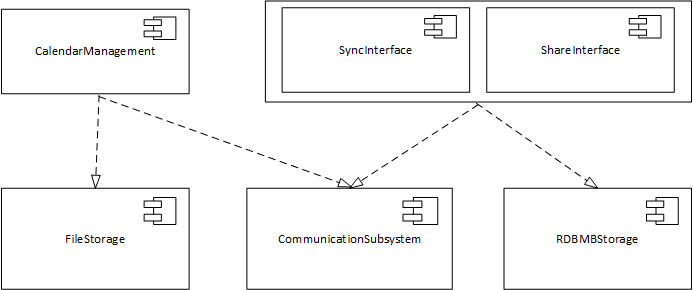
\includegraphics[width=135mm]{UMLComponentData.png}
\label{figur:UMLComponentData}
\end{figure}